\newcommand{\ImgProjectArhitecture}[1]{%
	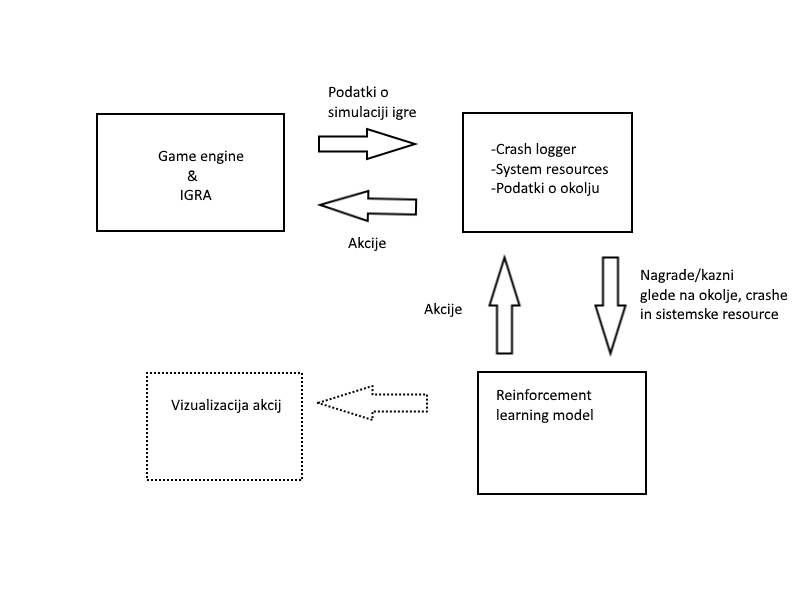
\includegraphics[scale=#1]{img/machine_learning/ShemaArhitekture.png}%
}

\chapter{Testiranje z strojnim učenjem}
TODO:
\begin{itemize}
    \item Narediti igro - osnovni 2D platformer z eno mehaniko
    \item Začet učit model z imitation learningom (zaradi hitrejšega začetka) in potem z reinforcement learningom~\cite{DBLP:journals/corr/abs-1803-05402}. Najprej bi ga naučil samo igrati igro in potem še doučil kako iskati napake
    \item Nagrajevanje modela, kjer so nagrade zelo redke~\cite{Ng99policyinvariance} in s pomocjo radovednos ter raziskovanje iskati napake v igri~\cite{pathakICMl17curiosity}. Funkcija nagrede bi bila vsota: verjetnosti za ne videno stanje, poraba spomina, poraba cpu, dolzina zadnjega frama. 
    \item Razlaga kako deluje Proximal Policy Optimization Algorithm (PPO)~\cite{DBLP:journals/corr/SchulmanWDRK17} v primerjavi z Trust Region Policy Optimization~\cite{DBLP:journals/corr/SchulmanLMJA15} in deep Q-network~\cite{deep-reinforcement-learning}
    \item uporaba Unity ML-agents frame worka~\cite{DBLP:journals/corr/abs-1809-02627} in dokumentacija~\cite{Unity-ML-Agents}
    \item Implementacija crash logerja, ki bi povedal ali vizualiziral zadnje akcije AI, koliko rama je bilo porablejno, koliko cpu je bilo uporabljeno, katera funkcija/vrstica je odletela.
    \item postopek testiranja AI:
    \begin{enumerate}
        \item postavitev okolja
        \item simulacija (dajanje rewardow, iskanje napake)
        \item cilj/rezultat (ce je AI ratalu dobimo nazaj sekvenco akcij in porabo spomina in cpu z lepimi grafi)
        \item povezetek -> predstavitev vseh rezultatov in popravki algoritma/funkcije
    \end{enumerate}
\end{itemize}

\ImgProjectArhitecture{0.5}